\section{Implementierung}

\subsection{Teilprojekte}


Die Solution ist in 3 Projekte aufgeteilt. Die App, die Domain und das Repository. In der App selbst ist das eigentliche Programm angesiedelt. Hier sind alle Views sowie ViewModels implementiert. Außerdem sind hier alle Konverter, welche Daten von einem ViewModel zur View, und umgekehrt, Konvertieren implementiert. In der Domain werden alle Models sowie das Interface zum Datenbankzugriff deklariert. Der Datenbankzugriff selber ist im Repository implementiert. Hier wird abgehandelt, wie Daten gespeichert werden. Durch die 3 Projekte soll eine Struktur entstehen, dass die App nur auf die Domain zugreifen kann. Die App greift auf die Datenbank nur über ein in der Domain deklariertes Interface auf das Repository zu. So wird realisiert, dass das Repository-Projekt ohne Probleme gegen ein anderes Ausgetauscht werden kann, welches das Interface zur Datenpersistierung implementiert. 

\subsection{Datenspeicherung}
Zur Datenspeicherung wird EntityFramework 6.2.0 mit einer SQL-Server Compact Edition genutzt. So ist eine leichte Portabilität gewährleistet. Wird das Programm portiert, und es ist keine Datenbank auf dem neuen System vorhanden, wird eine neue generiert. Der Datenbankzugriff erfolgt ausschließlich über das Interface \spitz{IPersistBookingsystemData}. In diesem sind alle Funktionen deklariert, die zum Datenaustausch mit der Datenbank benötigt werden. Implementiert wird dieses Interface im Projekt \spitz{Repository} von der Klasse \spitz{BookingSystemDataPersistence}. Diese ist als eine Art Database-Helper anzusehen. Die Models, welche in der Domain deklariert sind, werden nicht direkt in der Datenbank gespeichert. Hierzu gibt es für jedes Model ein Datenbank-Pendant. Zum Arbeitern mit der Datenbank werden Models in der \spitz{BookingSystemDataPersistenc} zur Speicherung erst in das Datenbankmodel geparst und umgekehrt.

\begin{figure}[h]
	\begin{center}
		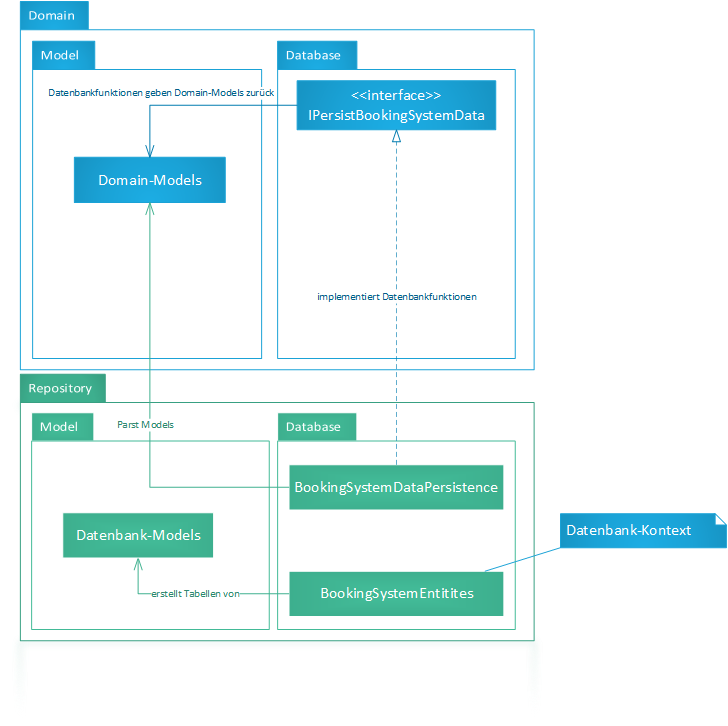
\includegraphics[width=\columnwidth]{Implementierung/Model-Datenbank.png}
	\end{center}
	\caption{Zusammenhang zwischen Domain und Repository}
	\label{fig:model-database}
\end{figure}

\subsection{Benutzerschnittstelle}
Die Benutzerschnittstelle wurde mit WPF implementiert. Hierzu wurde das MVVM-Pattern strikt durchgezogen. Einzig im \spitz{MainWindow} (einziges Fenster der Applikation) muss einmal Code-Behind verwendet werden um einen Daten-Kontext herzustellen. Ansonsten werden alle Interaktionen des Benutzers mit der Oberfläche durch ViewModels abgehandelt. 

Für das Layout wurde die Library MAHAPP.METRO verwendet. Dadurch wird leicht ein ansprechendes und flaches Design ermöglicht, welches dem Standarddesign von Windows ab Windows 8 stark ähnelt. Dadurch soll dem Nutzer ein Vertrautes Design vorgelegt werden.

Es wurde auf eine Menüleiste verzichtet, da diese zur Touch-Bedienung ungeeignet ist. Stattdessen wurde zur Navigation ein Hamburger-Menü genutzt.

\subsubsection{Navigation zwischen verschiedenen Ansichten}

Die Anzeige verschiedener Seiten im \spitz{MainWindow} wird ausschließlich durch UserControls umgesetzt. Hierfür wird eine bestimmte UserControl mit einem ViewModel verknüpft. Ändert sich in einem ViewModel eine Property, welche ein anderes ViewModel darstellt, ändert sich auch die View demensprechend. 
Als Beispiel: Das \spitz{MainWindow}, ausschnitt daraus zu sehen in Abbildung \ref{fig:mainWindow}, ist mit dem \spitz{MainViewModel}, ausschnitt zu sehen in Abbildung \ref{fig:mainViewModel}, verknüpft. Das \spitz{MainViewModel} besitzt eine Property \spitz{CurrentViewModel} vom Typ \spitz{BaseViewModel}. Ist das BaseViewModel vom Typ \spitz{BaseDataManagementViewModel} wird im dafür vorgesehenen Bereich die \spitz{BaseDataManagementView} angezeigt. Ist das \spitz{BaseViewModel} ein \spitz{RoomListViewModel} wird die \spitz{RoomListView} angezeigt. Dies wird, auch verschachtelt, in diesem Projekt angewandt. So wird automatisch durch Austausch des ViewModels auch die View geändert. 

\paragraph{Beispiel}

\begin{figure}[h]
	\begin{center}
		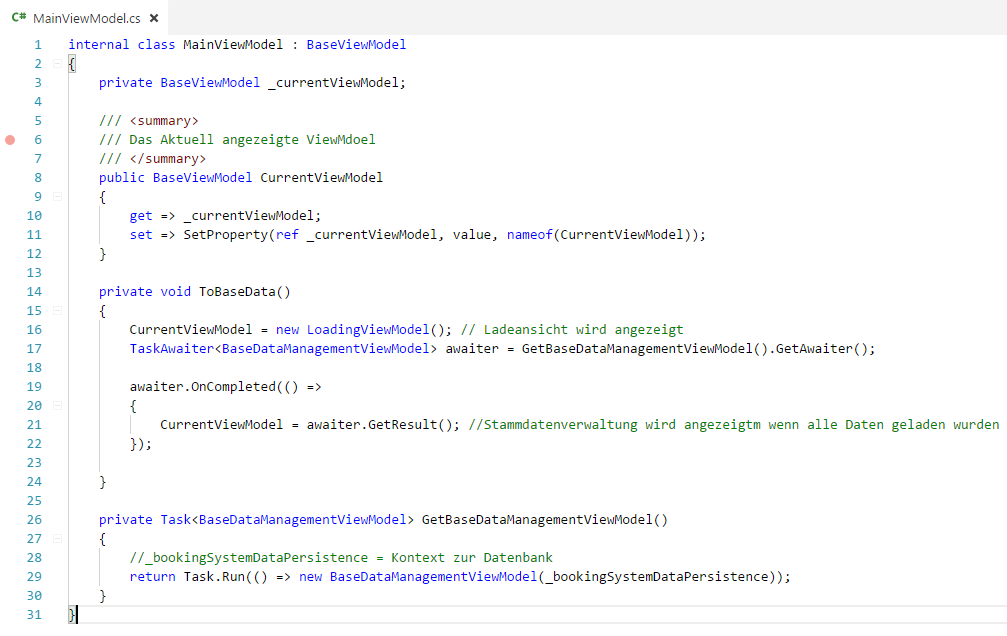
\includegraphics[width=\columnwidth]{Implementierung/MainViewModel.png}
	\end{center}
	\caption{Ausschnitt aus dem MainViewModel}
	\label{fig:mainViewModel}
\end{figure}

\begin{figure}[h]
	\begin{center}
		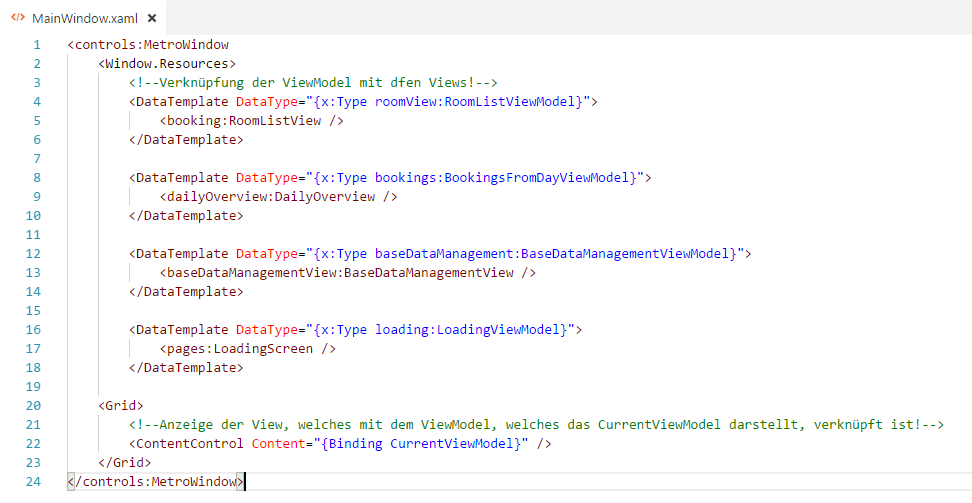
\includegraphics[width=\columnwidth]{Implementierung/MainWindow.png}
	\end{center}
	\caption{Ausschnitt aus dem MainWindow}
	\label{fig:mainWindow}
\end{figure}